% Created 2015-06-09 Tue 10:59
\documentclass[11pt]{article}
\usepackage[utf8]{inputenc}
\usepackage[T1]{fontenc}
\usepackage{fixltx2e}
\usepackage{graphicx}
\usepackage{longtable}
\usepackage{float}
\usepackage{wrapfig}
\usepackage{rotating}
\usepackage[normalem]{ulem}
\usepackage{amsmath}
\usepackage{textcomp}
\usepackage{marvosym}
\usepackage{wasysym}
\usepackage{amssymb}
\usepackage{hyperref}
\tolerance=1000
\author{Thierry BM}
\date{\today}
\title{Notes}
\hypersetup{
  pdfkeywords={},
  pdfsubject={},
  pdfcreator={Emacs 24.5.1 (Org mode 8.2.10)}}
\begin{document}

\maketitle
\tableofcontents


\section{Balbutiements}
\label{sec-1}

Plutôt que d'avoir une fonction d'utilité qui n'est de toute facon pas convexe, on peut
plutot tracer une fonction d'utilité qui vise un certain rendement. Ainsi, si on appelle
ce rendement r$_{\text{c}}$, l'utilité croît très rapidement lorsqu'elle se dirige à partir de la
gauche, alors qu'au contraire, lorsqu'elle s'en éloigne, ie. lorsqu'on observe des
rendements \emph{supérieurs} au rendement critique r$_{\text{c}}$, l'utilité décroit, mais beaucoup moins
rapidement.

On a ainsi un objectif qui est \emph{convexe}, et on a un problème qui somme toute est plus ciblé
autour d'un objectif précis. Si besoin est, on peut même raffiner l'utilité pour bien
définir comment on souhaite que la performance soit pénalisée ou non. 

On ajoute ensuite de la sélection de modèle à notre guise.

Maintenant qu'on obtient un \emph{q}, comment construire alors notre portefeuille? Pour chaque
stock, on obtient une proportion à investir, disons p$_{\text{s}}$. Disons qu'on désire investir dans
\emph{n} actifs différents, question de diversification, parmi \emph{m} actifs.

On peut ordonner les actifs par la valeur de q.x$_{\text{s}}$, car une valeur plus élevée indique
qu'on a davantage confiance dans ce stock pour fournir un rendement proche de notre
rendement idéal r$_{\text{c}}$.

On aura alors n proportions différentes (comprises pas tout à fait encore malheureusement)
entre 0 et 1. Supposons qu'on ait une suite \{p$_{\text{1}}$,p$_{\text{2}}$,\ldots{},p$_{\text{n}}$\} de proportions. On veut
construire un portefeuille avec tous ces actifs. Le portefeuille sera alors constitué
d'une proportion p$_{\text{1}}$ d'actifs risqués, et de l'actif sans risque. 

L'actif 2 sera alors constiué dans une proportion p$_{\text{2}}$ p$_{\text{1}}^{\text{2}}$, l'actif 3 dans une proportion
p$_{\text{3}}$p$_{\text{2}}$p$_{\text{1}}^{\text{2}}$. La règle de récurrence sera alors

p'$_{\text{i+1}}$ = p$_{\text{i+1 }}$p$_{\text{i}}$

et 

p'$_{\text{1}}$ = 1 - $\sum$$_{\text{i}\ge\ \text{2}}$$_$ p'$_{\text{i}}$

La valeur de m peut à nouveau être déterminée par sélection de modèle. 


\begin{itemize}
\item * *
\end{itemize}

\textbf{Le 19 avril 2015}

On travaille une utilité de la forme 

U(p) = $\alpha$$_{\text{1}}$(r$_{\text{c}}$ - p)$^{\text{ +}}$ + $\alpha$$_{\text{2}}$(p - r$_{\text{c}}$)$^{\text{ +}}$

où r$_{\text{c}}$ est le rendement souhaité. p est le rendement obtenu. On souhaite maximiser cette
utilité. 

Chaque stock s possède un vecteur d'informations x$_{\text{s}}$ déterminé à tous les jours. Notre
portefeuille est constitué de m actifs risqués et d'un actif sans risque. Donné q, le
rendement du portefeuille sur une période d'une journée est donné par

p$^{\text{m}}$(q) = p$_{\text{1}}$r$_{\text{1}}$ + p$_{\text{2}}$r$_{\text{2}}$ + $\cdots{}$ + p$_{\text{m}}$r$_{\text{m}}$ + (1 - $\sum$p$_{\text{i}}$) R$_{\text{f}}$

On détermine q avec le programme d'optimisation suivant:

max$_{\text{q}}$ $\sum$$_{\text{s}}$$\sum$$_{\text{t}}$ U(p$_{\text{st}}$(q))

Où ici 

p$_{\text{st}}$(q) = r$_{\text{st}}$ q$^{\text{T}}$x$_{\text{st}}$ + R$_{\text{f}}$(1 - q$^{\text{T}}$x$_{\text{st}}$)

On cherche donc à déterminer le vecteur q qui permettra de maximiser l'utilité \emph{sur tous}
\emph{les actifs, sur toutes les périodes}, autrement dit, un tel q permettrait de déterminer, en
moyenne l'allocation qui permettrait de se rapprocher d'un portefeuille de rendement r$_{\text{c}}$.

A x$_{\text{s}}$ on entend donc faire correspondre un \emph{rendement} r$_{\text{s}}$ à l'aide d'une fonction q(x$_{\text{s}}$) =
r$_{\text{s}}$. En somme, on considère que le rendement d'un certain actif ne serait pas uniquement
déterminé de facon intrinsèque mais serait alors déterminé à partir du vecteur
d'information x$_{\text{s}}$.

\begin{itemize}
\item * *
\end{itemize}


\section{\textbf{Le 20 avril 2015}}
\label{sec-2}

Revenons sur la nouvelle interprétation de q. Si par exemple on constitue de une base de
données constituée d'un seul actif, alors q fournira q.x$_{\text{s}}$ fournira la proportion à
investir si on vise un rendement r$_{\text{c}}$, donc

r q$^{\text{T}}$x$_{\text{s}}$ + R$_{\text{f}}$(1 - q$^{\text{T}}$x$_{\text{s}}$) = r$_{\text{c}}$

d'où on tire

q$^{\text{T}}$x$_{\text{s}}$ = (r$_{\text{c}}$ - R$_{\text{f}}$) / (r - R$_{\text{f}}$)

dont on peut se servir pour mesurer à quel point notre algorithme est efficace, ie. en
comparant les résultats empiriques avec ceux prédits par la théorie. 

Reste encore l'épineuse question de la normalisation, car pour certains attributs, chacun
peut possiblement se situer à des niveaux très différents. Aussi c'est pourquoi une
normalisation individuelle (par exemple recentré à la moyenne et réduit de $\rho$ écart types).

Par contre, on fait implicitementl'hypothèse que \emph{l'amplitude relative} des valeurs n'est
pas importante. Peut être y aurait il moyen de rajouter cette information dans x$_{\text{s}}$, sur une
colonne représentant pour chaque actif s'$\neq$s, la fraction d'amplitude. A voir. 

Une fois que nos données sont recentrées, on aura alors dans une proportion déterminée ($_{\text{à}}$
vérifier\_) des points tels que |x$_{\text{s}}$|$\le$1. Supposons qu'on préfère permettre une allocation
de portefeuille risquée comprise dans un intervalle [-$\alpha$, 1+$\alpha$], autrement dit on permet
dans une certaine mesure la vente à découvert et l'emprunt à R$_{\text{f}}$ pour obtenir davantage
d'exposition au marché. 

Si dans notre programme d'optimisation on emploie

q' = (1 + q)/2

\begin{itemize}
\item * *
\end{itemize}

La forme de la fonction d'utilité devient alors

U(p) = -$\beta$$_{\text{1}}$ Max(r$_{\text{c}}$ - p, 0) - $\beta$$_{\text{2}}$ Max(p - r$_{\text{c}}$, 0)

$\beta$$_{\text{1}}$ contrôle la pente de l'utilité pour des rendements inférieurs à r$_{\text{c}}$, $\beta$$_{\text{2}}$ contrôle la
pente pour des rendements supérieurs à r$_{\text{c}}$. On aura donc typiquement 

$\beta$$_{\text{1}}$ < $\beta$$_{\text{2}}$,

puisque des rendements supérieurs sont moins susceptibles d'affecter l'utilité.

Si p est fonction de q, par la fameuse relation

p(q) = r$_{\text{s}}$ q$^{\text{T}}$x$_{\text{s}}$ + R$_{\text{f}}$ (1 - q$^{\text{T}}$x$_{\text{s}}$)

alors on aura, au sens général, 

U(q) = -$\beta$$_{\text{1}}$ (r$_{\text{c}}$ - R$_{\text{f}}$ + q$^{\text{T}}$x$_{\text{s}}$(R$_{\text{f}}$ - r$_{\text{s}}$))$^{\text{+}}$ - $\beta$$_{\text{2}}$ (R$_{\text{f}}$ - r$_{\text{c}}$ + q$^{\text{T}}$x$_{\text{s}}$(r$_{\text{s}}$ - R$_{\text{f}}$))$^{\text{ +}}$

Si on lance un programme d'optimisation convexe de la forme

max$_{\text{q}}$ $\sum$$_{\text{s}}$$\sum$$_{\text{t}}$ U(q)
 sc. |q| $\le$ 1

Et qu'on suppose les vecteurs d'information x$_{\text{s}}$ normalisés, ie. |x$_{\text{s}}$| $\le$ 1, alors la
proportion comprise entre -1 et 1 (dans la plupart des cas). On voudrait que cette
proportion soit comprise entre [-$\alpha$, 1+$\alpha$].

Par exemple, si on pose $\alpha$=0, alors la transformation nécessaire pour obtenir un nouveau q
serait la suivante:

q' = (1 + q)/2

et ainsi on aurait la juste proportion d'investissement du portefeuille. 


\begin{itemize}
\item * *
\end{itemize}


\section{\textbf{Le 21 avril}}
\label{sec-3}

Choses restant à faire:

\begin{itemize}
\item Donner une période de dates lors de l'appel à x.
\item Rajouter un attribut pour représenter l'éloignement d'une certaine date.
\item \sout{Rajouter le prix moyen des n derniers jours}
\item Aller chercher de l'information sur le CA et sur le PDG. Par exemple, le genre et
l'âge du CEO (qu'on peut assumer être le premier dans la liste), et l'âge moyen et le
genre moyen des autres membres \emph{clés} (au sens de Yahoo).
\end{itemize}


\begin{itemize}
\item * *
\end{itemize}


\section{\textbf{Le 23 avril}}
\label{sec-4}

La question de la normalisation, toujours aussi épineuse. Voyons voir nos contraintes.

On veut que d'une part les attributs soient environ à la même échelle, pour que la
régularisation ait un sens. En effet, si par exemple on compare le volume quotidien de
vente, typiquement de l'ordre de 10$^{\text{6}}$, avec celui d'une volatilité sur 30 jours, de l'ordre
de 10$^{\text{-1}}$, naturellement l'ordre de grandeur des composantes de q ne sera pas semblable et
la normalisation sera alors biaisée.

Pour s'assurer qu'on travaille sur un ordre de grandeur commun, on pourrait alors préférer
recentrer tous les vecteurs d'information autour de la moyenne, puis ensuite réchelonner
selon la distance entre les valeurs extrêmes, de facon à avoir toutes les composantes du
nouveau vecteur réchelonné x' compris dans une boite de volume 1, ie.

\textasciitilde{}|x|$_{\text{1}}$ $\le$ 1

En pratique, on permet donc au vecteur d'information d'avoir une norme euclidienne L$_{\text{2}}$
supérieure à 1, mais toutefois assez proche.

Ceci permet également de construire une matrice sur laquelle on peut appliquer nos
nouveaux vecteurs d'information, afin d'en créer un vecteur de décision q.

Mais au fait de combien doit on les recentrer ces vecteurs d'informations? Car prenons par
exemple la colonne d'information pour un certain jour de la semaine. Ses valeurs
oscilleront entre 0 et 1, toutefois elles ne seront pas distribués uniformément puisque la
fonction donnant la valeur est une exponentielle. Donc sa moyenne ne tombera pas à 0.5
comme on aurait pu l'espérer. Faudrait il donc dans ce cas particulier les recentrer à
0.5?

A réfléchir\ldots{}

Bref, de toute facon nos mesures sont influencées par la présence du terme de biais,
présentement évalué à 1, mais qu'on aurait peut être avantage à changer pour une valeur
qui serait réchelonnée selon p, le nombre d'attributs.


\begin{itemize}
\item * *
\end{itemize}


\section{\textbf{Le 25 avril}}
\label{sec-5}

\begin{itemize}
\item Problème avec les jours. Ils n'atteignent pas 1!
\item Pourtant les semaines semblent bien fonctionner!
\end{itemize}

Ne pas oublier, si 

M $\in$ R$^{\text{m}\texttimes{}\text{n}}$

alors M est une matrice de m rangées et de n colonnes.

J'ai changé l'objectif pour y inclure un terme favorisant une norme \emph{élevée} pour
q. Soudainement on a un portefeuille qui se met à bouger davantage, ce qui est assez
encourageant. 

Supposons un taux annuel r$_{\text{a}}$. Alors le taux quotidien r$_{\text{q}}$ sera tel que

r$_{\text{q}}$ = log(1+r$_{\text{q}}$)/252

De la même facon, donné un taux quotidien r$_{\text{q}}$, le taux annuel correspondant sera 

r$_{\text{a}}$ = exp(252 r$_{\text{q}}$) - 1


\section{\textbf{Le 27 avril}}
\label{sec-6}

Notre dataset sera donc les trente éléments constituants le Dow Jones, et on remontera à
2009, car Visa ne commence qu'à partir de 2008. On fera une validation croisée à 5
plis. Donc, pour un test donné, le programme d'optimisation sera effectué sur 24 indices à
partir de 2009.

A présent comment faire les tests correctement? Puisqu'on peut interpéter q$^{\text{T}}$x comme une
certaine confiance statistique qu'on a dans un résultat, on pourrait alors décider de
choisir d'investir \emph{à chaque jour} dans le titre qui procure la valeur q$^{\text{T}}$x$_{\text{s}}$ la plus élevée,
et ainsi cumuler nos résultats, pas terriblement compliqué. On travaillerait alors sur un
portefeuille consitué de cinq actifs, dont un sans risque. 

Notons que cette décision pourrait également faire l'objet d'un changement, si on
considère qu'un autre algorithme plus efficace devrait être considéré.


\section{\textbf{Le 11 mai}}
\label{sec-7}

Bon, on est toujours à la recherche d'une borne théorique sur l'erreur qu'on peut faire
sur l'ensemble de test par rapport à l'ensemble d'entraînement. Dans le papier, R$_{\text{true}}$
représente alors l'espérance des coûts sur l'ensemble d'entraînement, alors que R\^{} est la
moyenne arithmétique sur l'ensemble de test. 

Et on cherche effectivement à minimiser la différence entre ces deux coûts: car si dans
notre cas on parvient à obtenir des rendements positifs avec notre politique q sur
l'ensemble d'entrainement, alors on voudrait avoir une garantie théorique que dans la
plupart des cas, notre politique appliquée à un ensemble de test performerait tout aussi
bien ou, du moins, aurait une performance dont l'ordre de comparaison avec ce qu'on aurait
obtenu avant serait mathématiquement connu.

\begin{itemize}
\item * *
\end{itemize}

\textbf{Rencontre avec Delage}

En somme, comment appliquer la notion de regret, soit à la construction de portefeuille,
soit à la construction du vecteur de décision. 

\begin{itemize}
\item * *
\end{itemize}

On a plusieurs problèmes à résoudre. D'abord la notion d'intervalle de confiance qui doit
être donnée et pour laquelle on souhaite réduire l'erreur sur notre utilité espérée sur
l'ensemble de test. 


\section{\textbf{Le 8 juin}}
\label{sec-8}

\uline{Quelques définitions (dans le cas \emph{newsvendor and portfolio})}

Le vrai risque:

R$_{\text{true}}$(q) = E$_{\text{D(x)}}$[C(q; D(x))]
        = E$_{\text{x}}$[E$_{\text{D(x)}}$[C(q; D(x))|x]]

Le risque empirique:

\^{}R(q;S$_{\text{n}}$) = 1/n $\sum$$_{\text{i}}$C(q, S$_{\text{n}}^{\text{i}}$)
         = 1/n $\sum$$_{\text{i}}$C(q, d$_{\text{i}}$(x$_{\text{i}}$))

"Since we desire the true risk to be low, a combination of low empirical risk and
sufficient stability ensures this."


Let X:R$^{\text{p}}$ be the information distribution, providing objects of the R$^{\text{p}}$ form, and let R(x):R
be the (real) distribution returns, and let D = R\texttimes{}X the \emph{information space}. 

\uline{Learning Algorith.}
A \emph{learning alogrithm} is a function whose argument is a dataset drawn from D$^{\text{n}}$, ie. with n
rows, mapping into the space of functions mapping from X to a portfolio space (to be
defined later) P. We shall denote this space of functions as X$^{\text{P}}$.

\uline{Loss of a decision vector q.}
The \emph{loss} l of a decision rule q $\in$ Q $\subset$ X$^{\text{P}}$ with respect to a sample d=(x,r) $\in$ D is defined as

l(q,d) = c(q(x),r(x))

for some cost function. 


Now how should this loss function be defined? On one hand we have the actual return of the
chosen stock. The real question here is when would the loss be zero. We always gain more
utility from higher return, and so if the chosen q gives us huge gains, then we cannot
claim that there's a single return at which the loss is completely absent. Our loss
function would therefore take the form of a decreasing exponential function exp(-$\mu$x).

But if we had such a loss function, we would then be out of line with a two-pieces linear
utility function. A log utility is of no use too, since its domain is only on R$_{\text{++}}$$_$. 

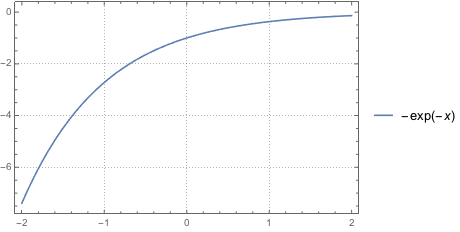
\includegraphics[width=.9\linewidth]{./Mai2015/FigExpUtility2.png}

But -exp(-$\mu$x) could be a good utility function, that can besides be scaled and moved
around using a parameter $\mu$ as an increasing rate. However we lose the insight developed
previously with the Newspaper article. 

The loss exp(-$\mu$x) is then perfectly in line with the utility and provide a reasonable
insight since the loss occured for higher return rates is much smaller than the loss
incured when dealing with higher return rates. 

We're also inline with the loss function of the newsvendor, since the loss we're trying to
minimize is now the same as the utility we're trying to maximize (modulo a minus sign).

In the newsvendor case, the loss the hypothesis q incurs on a random variate d=(x,r) drawn
from D, was defined as

l(q,d) = c(q(x),d)

where c was the newsvendors cost incurred from a demand d and an ordered quantity q(x). 

In our case, we again have not a situation where the loss is null, essentially because
we're in fact \emph{not} trying to predict the actual return rate, we instead try to form a good
portfolio from which we want to derive utility. The other problem, as mentioned
previously, is also that our utility has no supremum, ie. is not bounded above. In
pratical terms, this means that there's no single best decision that could have been made
had we known the return rate previously: if the rate was to be positive, then would have
massively borrowed to leverage the positive rate. On the other side, if the rate was
negative, then the reverse situation where we could have chosen between a mass short sale
or risk-free lending would have appropriate.

And in this sense, would there be no way to add a regularization term, ie. with which we
would discourage massive investments?

Here's a possible method to define l, but we first have to assume that ||q(x)||$_{\text{2}}^{\text{2}}$ $\le$ 1,
ie. the investment in the risky asset (under the two-assets portfolio hypothesis) is
bounded by 100\%, in financial terms, we cannot borrow money at R$_{\text{f}}$ to invest in the risky
asset. 

If r, ie. the return of the risky asset is above R$_{\text{f}}$, then we'll have wished we had
invested all our wealth in it, and thus the loss will be 

U(1,0) - U(q$^{\text{T}}$x, 1-q$^{\text{T}}$x)

if on the other hand the stock yields a return below R$_{\text{f}}$, then the reference will be the
utility derived from a perfectly safe portfolio, so that the loss becomes

U(0,1) - U(q$^{\text{T}}$x, 1-q$^{\text{T}}$x)

In either case, the loss is always positive (or at most zero).

\textbf{Note.} In the above expressions, U(x,y) represents the utility of a portfolio for which a
 proportion x is invested in the risky asset and y in the risk free asset.

According to Bousquet, an algorithm has $\beta$ uniform stability with respect to the loss
function l if for all dataset of m rows, we have the bound

`||l(q(S$_{\text{m}}$,d) - l(q(S'$_{\text{m}}$,d))||$_{\infty}$ $\le$ $\beta$$_{\text{m}}$

where q' is the hypothesis formed when removing a single row from S$_{\text{m}}$, the dataset (see
Bousquet p. 504 for total formalism). 

\textbf{Def.} An algorithm is uniformly stable if $\beta$$_{\text{m }}$$\le$ O(1/n).

\textbf{Def.} The \emph{generalization error} or the \emph{risk} depends on the training set S and the algorithm
 A$_{\text{S}}$ in the following way:

R(A$_{\text{S}}$,S) = E$_{\text{d}}$[l(A$_{\text{s}}$,d)]

\textbf{Def.} The \emph{empirical error} is the average of the loss over the training set S of m
elements:

$R_{emp}(A_S,S) = 1/m \sum_i l(A_s, d)$
% Emacs 24.5.1 (Org mode 8.2.10)
\end{document}